\chapter{Conclusiones y trabajos futuros}

En el marco de este proyecto se desarrolló la herramienta \emph{VMT} para la realización de espectáculos de \emph{video mapping} que implementa un enfoque novedoso, permitiendo la utilización de modelos tridimensionales para representar las superficies a proyectar y posibilitando la aplicación de efectos directamente sobre ellos. Cuenta con una interfaz de usuario interactiva en donde es posible visualizar los efectos en tiempo real a medida que se van diseñando.
Se lograron identificar etapas claramente diferenciadas en el proceso de creación de un espectáculo, lo cual fue muy útil para delinear requerimientos específicos para el desarrollo de \emph{VMT}. 

En las entrevistas que se mantuvieron con los \emph{VJs} éstos manifestaron un problema común que se da al utilizar más de un proyector cuyas proyecciones se solapan, causando deformaciones no deseadas en la visualización. \emph{VMT} mediante el soporte de múltiples proyectores evita este problema al tener control sobre qué objetos y efectos se muestran en cada proyector. Más en general, el manejo de múltiples proyectores distribuidos posibilita la creación de distintos esquemas de proyección soportando áreas amplias y disjuntas e incluso mapeos en 360 grados.

Los avances durante el transcurso del presente proyecto se han ido publicando en el \emph{blog}\cite{BLOG} elaborado para este propósito y permitiendo el seguimiento del mismo.
El código fuente de las aplicaciones, así como también otros materiales utilizados durante este proyecto se encuentran disponibles en los repositorios públicos \cite{SOURCEGOOGLE} y \cite{SOURCEGITHUB}.

\subsubsection{Obtención automática de la geometría}

Se logró resolver parcialmente el problema de reconstrucción automática de la escena a mapear mediante la implementación de una aplicación que toma una nube de puntos ya capturada, la procesa y genera un objeto tridimensional para luego ser utilizado por \emph{VMT}.
Se trabajó en el estudio de las técnicas y componentes existentes para la reconstrucción tridimensional de la escena, principalmente mediante la utilización del método de luz estructurada en donde se experimentaron varios problemas, la mayoría de ellos en la etapa de calibración del sistema cámara-proyector. 

Se logró realizar exitosamente una prueba de concepto del método de escaneo de Kyle McDonald \emph{Three-Phase shift}.
Si bien este método logra obtener una representación tridimensional, tiene limitantes en cuanto a que las superficies a escanear deben ser continuas y sin cambios bruscos en la profundidad. Es por esta razón que no es aplicable para obtener geometrías correspondientes a escenas comúnmente utilizadas en espectáculos de \emph{video mapping}, ya que en general éstas contienen objetos que no cumplen estas características.

\begin{figure}[H]
  \centering
    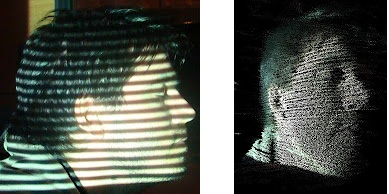
\includegraphics[width=0.7\textwidth]{./Cap7_conclusiones/Phase2.JPG}
  \caption[Imagen propia]{Izq: Patrón proyectado sobre sujeto de prueba. Der: Nube de puntos obtenida}
  \label{fig:cabeza}
\end{figure}

Se relevaron otros métodos de escaneo con luz estructurada que se adaptan mejor a un mayor rango de superficies, incluyendo las no soportadas por \emph{Three-Phase shift}, pero no se encontraron prototipos ya desarrollados para realizar pruebas de concepto y fue considerado fuera de los objetivos del proyecto.
Adicionalmente, durante el transcurso del proyecto surgió el dispositivo \emph{Kinect} para escanear objetos en tiempo real utilizando una implementación del método de luz estructurada. Con la liberación de su kit de desarrollo se incentivó su uso a desarrolladores de todo el mundo para una variedad de propósitos, lo que motivó a enfocar el alcance del proyecto en el procesamiento de nubes de puntos, independientemente de cómo estos puntos se obtienen, ya que \emph{Kinect} logra buenos resultados y es accesible en términos de costos.

Se implementó un prototipo de calibración tridimensional para obtener de forma automática la ubicación del proyector con respecto a una superficie.
Si bien este prototipo se pudo evaluar experimentalmente dando resultados que se aproximaban a lo esperado, necesitaba ajustes debido a las diferencias entre el funcionamiento de un proyector con el modelo ideal asumido. A su vez, el método de calibración se basa en parámetros intrínsecos del proyector como son su ángulo de enfoque el cuál debe ser medido experimentalmente, agregando errores a los cálculos.
En etapas posteriores del proyecto, al desarrollar la interfaz gráfica, se implementaron las transformaciones de cámaras virtuales mediante las cuales, si bien de forma manual, se puede lograr un ajuste más preciso.

\subsubsection{Espectáculos en vivo}

Se realizaron dos espectáculos en vivo con la herramienta \emph{VMT} en una versión alfa: el evento de cierre de Ingeniería de Muestra del año 2010\footnote{\url{http://www.fing.edu.uy/eventos/ingenieria_demuestra/2010/index.html}} de Facultad de Ingeniería de la Universidad de la República y un espectáculo durante la noche de fallos de fin de curso de Facultad de Arquitectura de la Universidad de la República.
\begin{figure}[H]
  \centering
    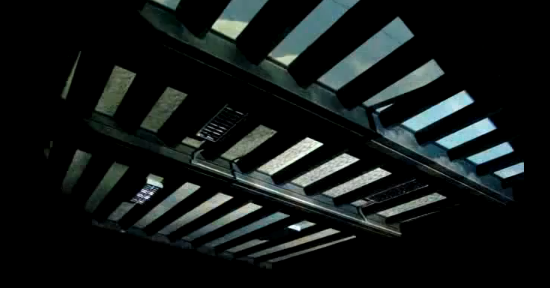
\includegraphics[width=0.7\textwidth]{./Cap7_conclusiones/ingMuestra1.png}
  \caption[Imagen propia]{Ingeniería de muestra 2010, \emph{quads} se iluminan al ritmo del audio.}
  \label{fig:ingMuestra1}
\end{figure}
\begin{figure}[H]
  \centering
    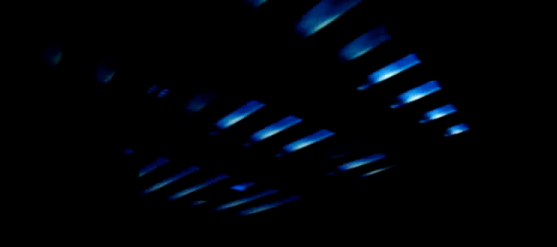
\includegraphics[width=0.7\textwidth]{./Cap7_conclusiones/ingMuestra2.png}
  \caption[Imagen propia]{Ingeniería de muestra 2010, videos en cada \emph{quad}.}
  \label{fig:ingMuestra2}
\end{figure}

\begin{figure}[H]
  \centering
    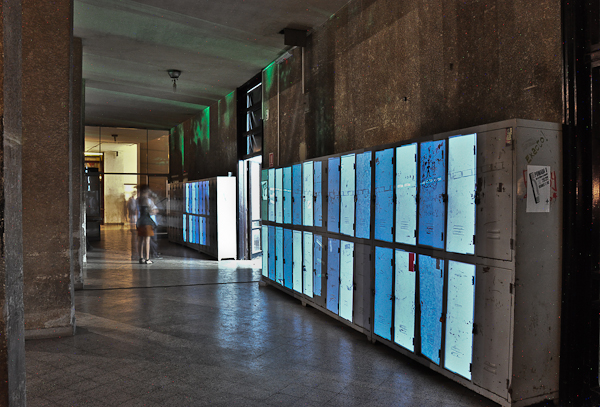
\includegraphics[width=0.7\textwidth]{./Cap7_conclusiones/Arqui1.jpg}
  \caption[http://www.farq.edu.uy/patio/conferencias-exposiciones-y-seminarios/noche-de-fallos-7.html]{Noche de fallos 2010, Fac. Arquitectura, casilleros iluminados.}
  \label{fig:Arquitectura1}
\end{figure}

\begin{figure}[H]
  \centering
    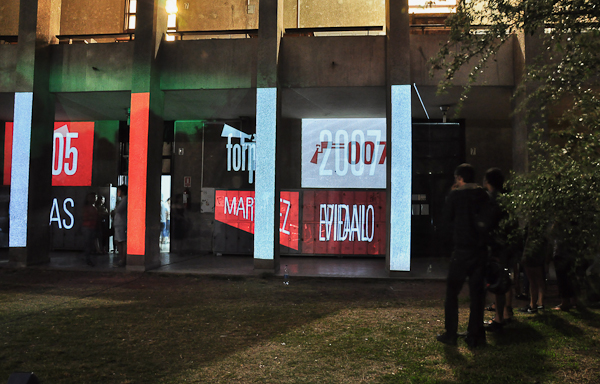
\includegraphics[width=0.7\textwidth]{./Cap7_conclusiones/Arqui2.jpg}
  \caption[http://www.farq.edu.uy/patio/conferencias-exposiciones-y-seminarios/noche-de-fallos-7.html]{Noche de fallos 2010, Fac. Arquitectura, casilleros y columnas iluminados.}
  \label{fig:Arquitectura2}
\end{figure}

\begin{figure}[H]
  \centering
    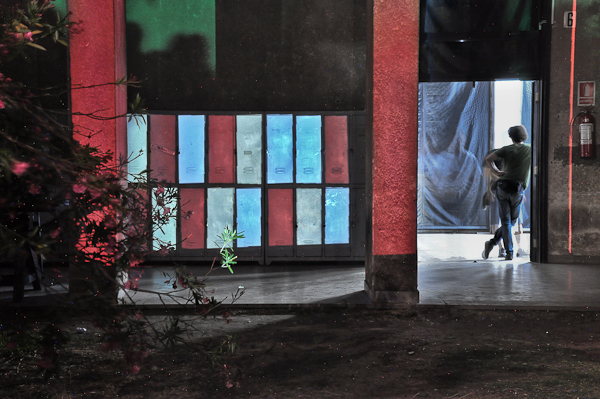
\includegraphics[width=0.7\textwidth]{./Cap7_conclusiones/Arqui3.jpg}
  \caption[http://www.farq.edu.uy/patio/conferencias-exposiciones-y-seminarios/noche-de-fallos-7.html]{Noche de fallos 2010, Fac. Arquitectura, casilleros y columnas cambiando de colores.}
  \label{fig:Arquitectura3}
\end{figure}

Durante la preparación y ejecución de los mismos se profundizó el conocimiento sobre lo necesario para llevar adelante un espectáculo de estas características, lo que ayudó a asentar las funcionalidades básicas que la aplicación debía cubrir. También se experimentó la importancia de la robustez y tolerancia a fallos que debe tener una aplicación que tiene como propósito la ejecución de espectáculos en vivo.

Desde el punto de vista funcional, se identificaron varios aspectos de la aplicación en las que se debía trabajar para mejorarlos, como ser el agregado de un mismo evento en varios momentos en la línea de tiempo, la agrupación de \emph{quads} para aplicarles el mismo efecto especificándolo una única vez y la ejecución del espectáculo a partir de un instante dado de la línea de tiempo. Todo lo anterior siendo accesible mediante una interfaz gráfica de usuario que adopte criterios comúnmente utilizados en aplicaciones orientadas al diseño.

En las instancias iniciales del desarrollo de la aplicación, se había decidido distribuir los archivos contenedores de la definición del espectáculo en todos los nodos esclavo de \emph{VMT}, enviando desde el nodo maestro únicamente órdenes para ejecutar los efectos en el instante requerido.
Esto presentaba varios problemas, por ejemplo durante la edición del espectáculo, ante cualquier modificación en los \emph{quads} u objetos tridimensionales era necesario actualizar el archivo de definición en cada nodo y posteriormente reiniciarlo.
Debido a esta fuerte limitación se rediseñó la arquitectura y el protocolo de comunicación entre nodos maestro y esclavo, centralizando la definición del espectáculo en el nodo \emph{VMT} maestro y soportando la creación de todos los elementos mediante nuevos mensajes que fueron agregados a dicho protocolo.
Estos mensajes envían a cada nodo esclavo los objetos bidimensionales, tridimensionales, grupos de objetos, y efectos necesarios para la visualización del espectáculo en ese nodo en particular.
De estas experiencias también surgió el inconveniente de pérdida de mensajes durante la ejecución debido al uso de redes inalámbricas. Estas redes proveen facilidades para conectar nodos debido a que no requieren cableado pero tienen una alta tasa de colisiones. En el caso de \emph{VMT}, el uso de estas redes provocó que la pérdida de mensajes durante la ejecución ocasionara un desfasaje en la reproducción en los diferentes nodos esclavo. Por ello se decidió utilizar para el espectáculo de Facultad de Arquitectura una red cableada \emph{Ethernet} y se observaron mejoras notorias en cuanto a la calidad de la transmisión sin notar pérdida de mensajes.

\subsubsection{Trabajo futuro}

Durante el transcurso del proyecto en sus etapas de investigación del estado del arte y desarrollo de la aplicación \emph{VMT}, así como también producto de la experiencia obtenida en los dos espectáculos en vivo mencionados, se identificaron varias oportunidades de mejora de lo realizado y de esto se desprendieron nuevas líneas de trabajo a seguir.

Un aspecto en donde hay posibilidades de mejoras es la ampliación de las funcionalidades brindadas por la interfaz gráfica de usuario para permitir un uso más directo e intuitivo de la aplicación.
Esto se puede lograr permitiendo posicionar y editar elementos bidimensionales y tridimensionales directamente mediante acciones de ratón, sin dejar de soportar la opción de posicionamiento mediante el ingreso de coordenadas ya que esto permite un control más preciso.

\emph{VMT} permite únicamente utilizar \emph{quads} para representar figuras bidimensionales. Esto provoca que de necesitarse modelar figuras con más vértices para cubrir una superficie compleja sea necesario construirla utilizando más de un \emph{quad}. Una mejora posible sería permitir definir figuras bidimensionales con más de cuatro vértices para simplificar la definición en estos casos. Esto tiene la dificultad de que el mapeo de texturas no es directo para figuras con más de cuatro vértices por lo que la aplicación debería proveer un mecanismo para definir las coordenadas de mapeo para cada vértice. De todas formas, esta funcionalidad se puede cubrir mediante el uso de objetos \emph{3DS} que ya incorporen las coordenadas de mapeo en los vértices.

Para el manejo de objetos tridimensionales, \emph{VMT} depende de herramientas externas que permitan el manejo de archivos \emph{3DS}. En particular, las tareas que serían deseables incluir en \emph{VMT} son las de edición de vértices y caras de mallas tridimensionales y asignación de materiales a grupos de caras.

Actualmente \emph{VMT} no dispone de una interfaz visual que asista a la sincronización de la ejecución de los efectos visuales con el audio que acompaña el espectáculo.
Una forma en que esto podría realizarse es desplegando una visualización de la onda de audio, para tener una idea de en qué instantes se provocan cambios importantes en el sonido y asignar efectos directamente en los instantes visualizados.

Por último, debido al amplio estudio en métodos de obtención automática de geometría tridimensional y a la más reciente liberación del kit de desarrollo de \emph{Kinect} sería de interés integrar la captura de geometría con \emph{VMT} para permitir un uso más dinámico de la aplicación, completando de esta forma el ciclo de trabajo para la construcción de un espectáculo de \emph{video mapping}.
